\section{Connectedness} 

\subsection{Connected Spaces}

  \begin{definition}[Separation]
    Let $X$ be a topological space. A \textbf{separation} of $X$ is a pair $U, V$ of disjoint nonempty open subsets of $X$ whose union is $X$. The space $X$ is said to be \textbf{connected} if it satisfies the equivalent definitions 
    \begin{enumerate}
      \item there does not exist a separation of $X$. 
      \item the only subsets of $X$ that are clopen in $X$ are the empty set and $X$ itself. 
    \end{enumerate}

    \begin{figure}[H]
      \centering 
      \begin{tikzpicture}[scale=1.2]
        % First diagram - disjoint sets
        \begin{scope}
          % Set A
          \draw[dashed, thick] plot [smooth cycle, tension=0.8] 
            coordinates {(-1.5,1) (-0.5,1.3) (0,0.5) (-0.8,-0.2) (-1.8,0.3)};
          \node at (-1,0.5) {$A$};
          
          % Set B
          \draw[dashed, thick] plot [smooth cycle, tension=0.8] 
            coordinates {(1,0) (1.8,0.2) (1.5,-0.8) (0.5,-0.6)};
          \node at (1.2,-0.3) {$B$};
        \end{scope}
        
        % Second diagram - sets with common boundary
        \begin{scope}[xshift=6cm]
          % Set A - upper portion with less rounding
          \draw[dashed, thick] 
            plot [smooth cycle, tension=0.0] 
            coordinates {(-1,1) (0,1.5) (1,1) (1,0) (-1,0)};
          \node at (0,0.7) {$A$};
          
          % Set B - lower portion with less rounding
          \draw[dashed, thick] 
            plot [smooth cycle, tension=0.0] 
            coordinates {(-1,0) (1,0) (0.5,-1) (-0.5,-1)};
          \node at (0,-0.5) {$B$};
        \end{scope}
      \end{tikzpicture}
      \caption{Two examples of spaces $X = A \sqcup B$ that are not connected. In the right, $A$ and $B$ overlap in their boundary but are not connected since they are open. } 
      \label{fig:separation}
    \end{figure}
  \end{definition}

  Connectedness is clearly a topological property since it is completely defined in terms of the collection of open sets in $X$. Since homeomorphisms preserves topological properties, we can say that if $X$ is connected, every space homeomorphic to $X$ is also connected. 

  \begin{example}[Separation of a Rectangle]
    The space $Y = (0,1) \times (0,1) \cup (1,2) \times (0,1) \subset \mathbb{R}^2$ has the clear separation 
    \begin{equation}
      (0, 1) \times (0, 1) \text{ and } (1, 2) \times (0, 1)
    \end{equation}

    \begin{figure}[H]
      \centering 
      \begin{tikzpicture}[scale=1.5]
        \draw[dashed] (0,0) rectangle (2,1);
        \draw[dashed] (1,1)--(1,0);
      \end{tikzpicture}
      \caption{We can visualize the separation of $Y$ as such. } 
      \label{fig:separation_of_rectangle}
    \end{figure}
    Note that the dashed line is not in $Y$. Even though the dashed line contains limit points of both the left and right subset of $Y$, this does not matter. 
  \end{example}

  \begin{example}
    Let $X$ denote a two-point space in the indiscrete topology. Clearly, there is no separation of $X$, so $X$ is connected. 
  \end{example}

  \begin{example}
    Let $Y$ denote the subspace $[-1,0) \cup (0,1]$ of $\mathbb{R}$. Each of the sets $[-1,0)$ and $(0,1]$ is nonempty and open in $Y$ (but not in $\mathbb{R}$), so they form a separation of $Y$. Also, note that neither of these sets contains a limit point of the other (even though they have a common limit point $0$). 
  \end{example}

  \begin{example}
    $[-1,1]$, the subspace of $\mathbb{R}$, has no separation, so it is connected. 
  \end{example}

  \begin{example}
    The rationals $\mathbb{Q} \subset \mathbb{R}$ are not connected since given any irrational number $a$, we can write $Y$ as the union of sets
    \begin{equation}
      Y \cap (-\infty, a), \; Y \cap (a, +\infty)
    \end{equation}
    which are open in the subspace topology. 
  \end{example}

  \begin{lemma}
    If the sets $C$ and $D$ form a separation of $X$, and if $Y$ is a connected subset of $X$, then $Y$ lies entirely within either $C$ or $D$. 
  \end{lemma}
  \begin{proof}
    Trivial. Easy to visualize. 
  \end{proof}

  \begin{theorem}
    The union of a collection of connected sets that have a point in common is connected. 

    \begin{figure}[H]
      \centering 
      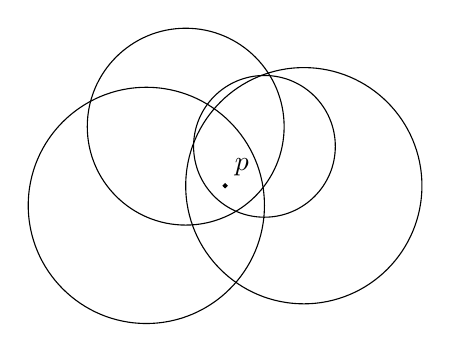
\begin{tikzpicture}[scale=0.5]
        \draw[fill] (0,0) circle (0.05);
        \node[above right] at (0,0) {$p$};
        \draw (1,1) circle (1.8);
        \draw (-1,1.5) circle (2.5);
        \draw (-2, -0.5) circle (3);
        \draw (2,0) circle (3);
      \end{tikzpicture}
      \caption{We can visualize this by thinking of overlapping balls. } 
      \label{fig:overlapping_circles}
    \end{figure}
  \end{theorem}
  \begin{proof}
    Let $\{A_\alpha\}$ be a collection of connected subsets of a space $X$, and let 
    \begin{equation}
      p \in \bigcap A_\alpha
    \end{equation}
    Then, we claim that 
    \begin{equation}
      Y \equiv \bigcup A_\alpha
    \end{equation}
    is connected. Assume $Y$ is not connected, that is, there exists $Y = C \cup D$ as a separation of $Y$. Then, $p \in C$ or $p \in D$. Without loss of generality, suppose $p \in C$. Since each $A_\alpha$ is connected, it must lie entirely within $C$ (by the previous lemma, since it contains the point $p \in C$) $\implies D = \emptyset$, a contradiction that $D$ must be nonempty. 
  \end{proof}

  \begin{theorem}
    Let $A$ be a connected subset of $X$. If $A \subset B \subset \bar{A}$, then $B$ is also connected. 
  \end{theorem}
  \begin{proof}
    Assume $B = C \cup D$ is a separation of $B \implies A$ must lie entirely within $C$ or $D$. Without loss of generality, suppose $A \subset C$, which implies that $\bar{A} \subset \bar{C}$. Since $\bar{C}$ and $D$ are disjoint, $B$ cannot intersect $D \implies D = \emptyset$, a contradiction. Therefore, there exists no separation of $B$. 
  \end{proof}

  \begin{theorem}
    The image of a connected space under a continuous map is connected. 
  \end{theorem}
  \begin{proof}
    Let $f: X \longrightarrow Y$ be a continuous map, and let $X$ be connected. We wish to prove that the image set $Z = f(X)$ is also connected. Let us denote the restriction of $f$ to $Z$ as
    \begin{equation}
      \Tilde{f}: X \longrightarrow Z
    \end{equation}
    which is continuous and surjective. We prove by contradiction. Assume that $Z = A \cup B$ is a separation of $Z$ into 2 disjoint nonempty open sets. Then, $\Tilde{f}^{-1} (A)$ and $\Tilde{f}^{-1}(B)$ are disjoint open sets whose union is $X \implies \Tilde{f}^{-1} (A) \cup \Tilde{f}^{-1}(B)$ form a separation of $X$. This contradicts the hypothesis that $X$ is connected $\implies Z$ is connected.  
  \end{proof}

  \begin{theorem}
    Given connected topological spaces $X_\alpha$ with $\alpha \in J$, the Cartesian products of them is connected. That is, 
    \begin{equation}
      \prod_{\alpha \in J} X_\alpha
    \end{equation}
    with the product topology is connected. If $J$ is infinite, then the product space is not necessarily connected under the box topology. 
  \end{theorem}

  \begin{definition}[Linear Continuum]
    A simply ordered set $L$ having more than one element is called a \textbf{linear continuum} if the following hold. 
    \begin{enumerate}
      \item $L$ has the least upper bound property. 
      \item If $x <y$, then there exists $z$ such that $x<z<y$
    \end{enumerate}
    A classic example of the linear continuum is the real number line and every set homeomorphic to it. 
  \end{definition}

  \begin{theorem}
    If $L$ is a linear continuum in the order topology, then $L$ is connected and so it every interval and ray in $L$. 
  \end{theorem}

  \begin{corollary}
    $\mathbb{R}$ is connected, along with every interval and ray in $\mathbb{R}$. 
  \end{corollary}

  \begin{theorem}[Intermediate Value Theorem]
    Let $f: X \longrightarrow Y$ be a continuous map of the connected space $X$ into the ordered set $Y$, with the order topology. Given $a, b \in X$ and $r \in Y$ such that $f(a)<r<f(b)$, then there exists a point $c \in X$ such that $f(c) = r$. 
  \end{theorem}
  \begin{proof}
    Assuming the hypothesis, the sets 
    \begin{equation}
      A \equiv f(X) \cap (-\infty, r), \; B \equiv f(X) \cap (r, +\infty)
    \end{equation}
    are disjoint. They are also nonempty since 
    \begin{equation}
      f(a) \in A, \; f(b) \in B
    \end{equation}
    $A$ and $B$ are open since they are the intersection of open sets. Now, assume that there exists no point $c \in X$ such that $f(c) = r$. Then, 
    \begin{equation}
      f(X) = A \cup B
    \end{equation}
    would define a separation of $X$, contradicting the fact that the image of a connected space under a continuous map must be connected. Therefore, $c$ exists. 
  \end{proof}

\subsection{Path Connectedness}

  \begin{definition}[Path Connectedness]
    Given points $x$ and $y$ of the space $x$, a \textbf{path} in $X$ from $x$ to $y$ is a continuous map $f: [a,b] \longrightarrow X$ of some closed interval in $\mathbb{R}$ to $X$ such that $f(a) = x$ and $f(b)=y$. A space $X$ is said to be \textbf{path connected} if every pair of points of $X$ can be joined by a path in $X$. 
  \end{definition}

  \begin{proposition}[Path Connectedness implies Connectedness]
    $X$ is path connected $\implies X$ is connected. 
    \begin{figure}[H]
      \centering 
      \begin{tikzpicture}[scale=0.5]
        \draw[dashed] (5,1) circle (2);
        \draw[dashed] (0,0) circle (2);
        \node at (-1,-1) {$C$};
        \node at (6,2) {$D$};
        \draw plot [smooth] coordinates {(0,0) (2,1.5) (4.5,2)};
        \draw[fill] (0,0) circle (0.05);
        \draw[fill] (4.5,2) circle (0.05);
        \node at (-4,1) {$X = C \cup D$};
      \end{tikzpicture}
      \caption{}  
      \label{fig:path_vs_reg_connectedness}
    \end{figure}
  \end{proposition}
  \begin{proof}
    $X$ not connected implies that there exists disjoint open subsets $C, D$ such that $C \cup D = X$. Assume that $X$ is path connected, i.e. there exists a continuous function $g: [0,1] \longrightarrow X$. Then the preimage of $C$ and $D$ in $X$ must be open sets $g^{-1} (C), g^{-1} (D) \subset [0,1]$ such that $g^{-1}(C) \cup g^{-1}(D) = [0,1]$. But this isn't possible since $[0,1]$ is connected, so by contradiction, $X$ is not path connected. The contrapositive of this statement results in the proposition. 
  \end{proof}

  However, note that $X$ connected $\centernot\implies$ $X$ path connected. Note the following example. 

  \begin{example}[Connected but Not Path Connected]
    Given the following function 
    \begin{equation}
      f:[0,1] \longrightarrow [-1,1], \; f(x) = \sin{\frac{1}{x}}
    \end{equation}
    $[-1,1]$ is connected, but not path connected since the path oscillates infinitely many times as it approaches $0$ from both $-1$ and $1$. 
  \end{example}

  The concept of homotopies is dealt with in algebraic topology, but it is worthwhile to mention it now. 

  \begin{definition}[Homotopy]
    Two continuous paths from $x$ to $y$ in topological space $X$ is \textbf{homotopic} if one can be continuously "deformed" into the other, such a deformation being the \textbf{homotopy} between two functions. The set of linearly homotopic paths form a relation, and thus \textbf{homotopy classes} can be further defined. 
    \begin{figure}[H]
      \centering 
      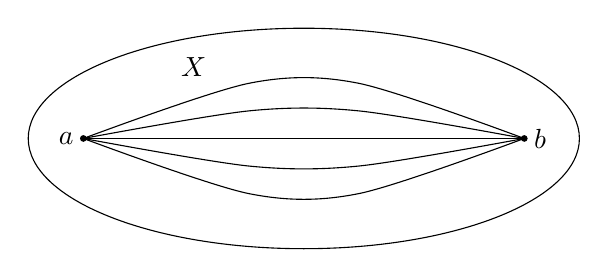
\begin{tikzpicture}[scale=0.7]
        \draw (0,0) ellipse (5 and 2);
        \draw[fill] (-4,0) circle (0.05);
        \draw[fill] (4,0) circle (0.05);
        \draw plot [smooth] coordinates {(-4,0) (-1,1) (1,1) (4,0)};
        \draw (-4,0)--(4,0);
        \draw plot [smooth] coordinates {(-4,0) (-1,0.5) (1,0.5) (4,0)};
        \draw plot [smooth] coordinates {(-4,0) (-1,-0.5) (1,-0.5) (4,0)};
        \draw plot [smooth] coordinates {(-4,0) (-1,-1) (1,-1) (4,0)};
        \node at (-2,1.3) {$X$};
        \node[left] at (-4,0) {$a$};
        \node[right] at (4,0) {$b$};
      \end{tikzpicture}
      \caption{Visually, the set of all the curves in the space $X$ as shown are in a single homotopy class.} 
      \label{fig:single_homotopy_class}
    \end{figure}
  \end{definition}

  It is clear that the space $X$ consists of a single homotopy class of curves from $a$ to $b$. However, a space may have an infinite number of such classes. 

  \begin{figure}[H]
    \centering 
    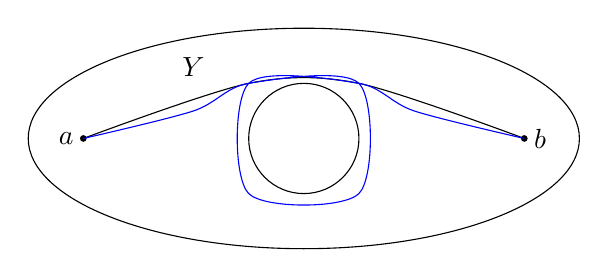
\begin{tikzpicture}[scale=0.7]
      \draw (0,0) ellipse (5 and 2);
      \draw[fill] (-4,0) circle (0.05);
      \draw[fill] (4,0) circle (0.05);
      \draw plot [smooth] coordinates {(-4,0) (-1,1) (1,1) (4,0)};
      \node[left] at (-4,0) {$a$};
      \node[right] at (4,0) {$b$};
      \draw (0,0) circle (1);
      \node at (-2,1.3) {$Y$};
      \draw[blue] plot [smooth] coordinates {(-4,0) (-2,0.5) (-1,1) (1,1) (1,-1) (-1,-1) (-1,1) (1,1) (2,0.5) (4,0)};
    \end{tikzpicture}
    \caption{Let us define the space $Y \equiv X \setminus C$ where $C$ is a circular region in $X$. Then, $Y$ has an infinite number of homotopy classes. We show two curves, that are in two different homotopy classes. }
    \label{fig:homotopy_class}
  \end{figure}

  \begin{definition}[Simply Connected Set]
    A \textbf{simply connected set} is a set such that all paths between any two given points are homotopic. That is, a simply connected set has one homotopy class. 
  \end{definition}

\subsection{Components and Path Components}

  \begin{definition}[Connected Components]
    Given $X$, define an equivalance relation on $X$ by setting $x \sim y$ if there is a connected subset of $X$ containing both $x$ and $y$. The equivalence classes are called the \textbf{components}, or \textbf{connected components}, of $X$. 
  \end{definition}

  \begin{theorem}
    The components of $X$ are connected disjoint subsets of $X$ whose union is $X$, such that each connected subset of $X$ intersects only one of them. 
  \end{theorem}
  \begin{proof}
    Trivial. 
  \end{proof}

  \begin{definition}[Path Components]
    We can define another equivalence relation on the space $X$ by defining $x \sim y$ if there is a path in $X$ from $x$ to $y$. The equivalence classes are called the \textbf{path components} of $X$. It can be easily shown that this is an equivalence relation. 
  \end{definition}

  \begin{theorem}
    The path components of $X$ are path connected disjoint subsets of $X$ whose union is $X$, such that each path connected subset of $X$ intersects only one of them. 
  \end{theorem}
  \begin{proof}
    Trivial.
  \end{proof}

  The property of local connectedness is also important for a space to possess. Roughly speaking, local connectivity means that each point has "arbitrarily small" neighborhoods that are connected. 

  \begin{definition}[Locally Connected at a Point]
    A space $X$ is said to be \textbf{locally connected at $x$} if for every neighborhood $U$ of $x$, there is a connected open neighborhood $V$ of $x$ contained in $U$. If $X$ is locally connected at all of its points, then $X$ is simply said to be \textbf{locally connected}. 

    \begin{figure}[H]
      \centering 
      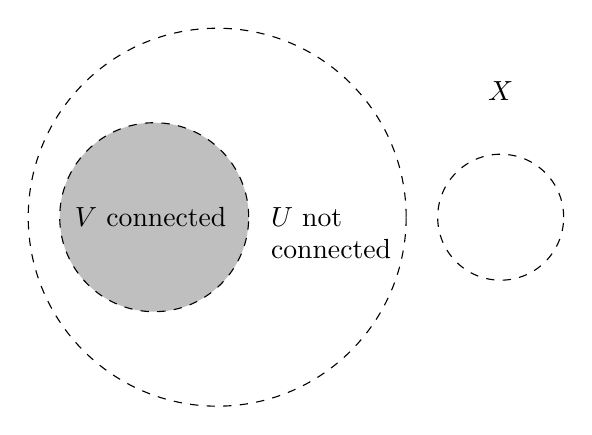
\begin{tikzpicture}[scale=0.8]
        \draw[fill] (-2,0) circle (0.05);
        \node[above] at (-2,0) {$x$};
        \draw[dashed] (-1.5,0) circle (3);
        \draw[dashed] (3,0) circle (1);
        \draw[dashed, fill=lightgray] (-2.5,0) circle (1.5);
        \node[left] at (-1.2,0) {$V$ connected};
        \node[right] at (-0.8,0) {$U$ not};
        \node[right] at (-0.8,-0.5) {connected};
        \node at (3,2) {$X$};
      \end{tikzpicture}
      \caption{Visually, in the space $X$, let $U$ be the union of the two open balls shown below. $U$ is clearly open, but not necessarily connected. However, we can form a  neighborhood $V$ of $x$ contained in $U$ such that $V$ is connected. }
      \label{fig:locally_connected}
    \end{figure}
  \end{definition}

  Equivalently, $X$ is locally connected if there exists a basis for $X$ consisting of connected sets. Local connectedness and connectedness of a space are independent of each other. 

  \begin{definition}[Locally Path Connected at a Point]
    A space $X$ is \textbf{locally path connected at $x$} if for every neighborhood $U$ of $x$, there is a path connected neighborhood $V$ of $x$ completely contained in $U$. If $X$ is locally path connected at each of its points, then it is simply said to be \textbf{locally path connected}. We can visualize this condition similarly as that of local connectedness. 
  \end{definition}

  \begin{theorem}
    A space $X$ is locally connected if and only if for every open set $U$ of $X$, each component of $U$ is open in $X$. 
  \end{theorem}
  \begin{proof}
    We prove bidirectionally. 
    \begin{enumerate}
      \item $(\rightarrow)$ Suppose that $X$ is locally connected. Let $U$ be an open set of $X$ and let $C$ be a component of $U$. If $x$ is any point in $C$, by definition of local connectedness, there exists a connected neighborhood $V$ of $x$ fully contained in $U$. Since $V$ is connected, it must additionally lie completely within $C \implies C$ is open in $X$. 
      \item $(\leftarrow)$ Suppose that the components of open sets in $X$ are open. Given a point $x \in X$ and neighborhood $U$ of $x$, let $C$ be the component of $U$ containing $x$, which means that $C$ is connected. By hypothesis, the components of open sets are alsvo open, so $C$ is also open. Since an open, connected set $C$ exists for all $x \in X$, $X$ is locally connected. 
    \end{enumerate}
  \end{proof}

  \begin{theorem}
    A space $X$ is locally path connected if and only if for every open set $U$ of $X$, each path component of $U$ is open in $X$.
  \end{theorem}

  \begin{theorem}
    If $X$ is a topological space, each path component of $X$ lies in a component of $X$. If $X$ is locally path connected, then the components and the path components of $X$ are the same. 
  \end{theorem}

